\documentclass[tikz,border=10pt]{standalone}
\usetikzlibrary{decorations.markings,quotes}
\begin{document}
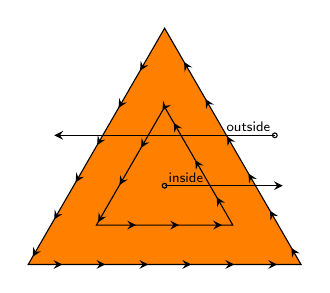
\begin{tikzpicture}[
    draw=black, fill=orange,
    decoration={markings, 
    mark=  between positions 0.04 and 1 step 0.035 
        with {\arrow{stealth}}},
    every edge quotes/.style = {font=\sffamily\tiny,sloped,above,inner sep=1pt}
     ]
  \filldraw[postaction={decorate}] (90:2) -- (210:2) -- (330:2) -- cycle
        (90:1) -- (210:1) -- (330:1) -- cycle;
  \draw (0,0) circle[fill=black,radius=0.03] edge[-stealth,"inside" pos=0.18] (1.5,0);
  \draw (1.4,0.64) circle[fill=black,radius=0.03] edge[-stealth,"outside" pos=0.12] (-1.4,0.64);
\end{tikzpicture}
\end{document}
